\chapter{Implementacja}
W niniejszym rozdziale opisano proces, którego celem było zaimplementowanie platformy spełniającej postawione wcześniej wymagania funkcjonalne oraz niefunkcjonalne. 
W procesie tym wystąpiły wszystkie kluczowe kroki, począwszy od konfiguracji środowiska, przez rozwój aplikacji backendowej i frontendowej, aż po integrację z systemami zewnętrznymi oraz konfigurację kontenerów Dockerowych. Lektura tego rozdziału powinna pozwolić na zapoznanie się ze szczegółami implementacji, uwagami dotyczącymi użytych technologii, narzędzi oraz metodami, które umożliwiły realizację tak założonego projektu.

W rozdziale omówione zostaną aspekty techniczne implementacji, w tym struktura repozytoriów kodu, konfiguracja środowiska developerskiego, użyte frameworki i biblioteki, oraz zagadnienia związane z budową i wdrożenia aplikacji. Zaznaczono w nim główne decyzje architektoniczne, które wpłynęły na projektowanie aplikacji oraz integrację z systemami zewnętrznymi, w tym bazami danych, serwerami aplikacji oraz kontenerami Dockerowymi.

Podczas implementacji, szczególną uwagę poświęcono skalowalności aplikacji, zapewnieniu bezpieczeństwa danych oraz optymalizacji wydajności. Każdy z komponentów systemu – zarówno backend jak i frontend – został zaprojektowany w sposób umożliwiający łatwą rozbudowę oraz integrację z dodatkowymi usługami w przyszłości.


\section{Podział logiczny}
\subsection{Komponenty systemu}
Zgodnie z założeniami co do architektury, podczas implementacji stworzono główne moduły systemu: frontend oraz backend (patrz podrozdział~\ref{subsec:ZarysArchitektury}).\\[-10pt]

\noindent \textbf{Frontend} -- %zbudowany w React jako aplikacja wielostronicowa (MPA), % to już było w założeniach ogólnych
odpowiada za prezentację danych i interakcję z użytkownikami. Podzielono go na moduły odpowiadające różnym domenom funkcjonalnym. Moduł blockchain prezentuje dane związane z blockchainami Bitcoin, Ethereum i Solana, w tym szczegóły transakcji, bloków oraz kont. Ten moduł zawiera podkomponenty obsługujące wyszukiwanie oraz wyświetlanie szczegółowych informacji. Moduł kryptowalut zarządza kategoriami kryptowalut, danymi historycznymi, rynkiem globalnym oraz rankingami. Dodatkowo frontend oferuje widoki użytkownika, takie jak logowanie, rejestracja oraz strona główna. Komunikacja z backendem odbywa się za pomocą biblioteki axios, z uwierzytelnianiem opartym na tokenach JWT przechowywanych w \texttt{localStorage}.\\[-10pt]

\noindent \textbf{Backend} -- %zaimplementowany w Spring Boot 3 przy użyciu Javy 21 % to już było w założeniach ogólnych
jest centralnym komponentem systemu. Integruje funkcje związane z logiką biznesową, bazą danych oraz zewnętrznymi dostawcami informacji. Backend udostępnia API REST dla frontendu i obsługuje kilka kluczowych domen, takich jak kryptowaluty, NFT oraz zasoby zewnętrzne. Moduł kryptowalut oferuje funkcje zarządzania kategoriami, danymi historycznymi oraz danymi rynkowymi. Moduł NFT zarządza tokenami, kolekcjami oraz ich statystykami. Backend również integruje dane blockchainowe, takie jak transakcje i bloki, które są dynamicznie pobierane z zewnętrznych API, takich jak Etherscan czy CoinMarketCap. Ponadto backend wywołuje dedykowane skrypty w Node.js w celu realizacji zaawansowanych operacji blockchainowych, takich jak symulacje transakcji i airdropy oraz skrypt w kontenerze Pythonowym, tak aby uzyskać dane o cenie kryptowalut na dany dzień.

Część backendu odpowiada również za bezpieczeństwo, realizowane poprzez mechanizm OAuth2 i tokeny JWT. Tokeny te są wykorzystywane do uwierzytelniania użytkowników oraz zabezpieczania komunikacji między frontendem a backendem. W backendzie baza danych PostgreSQL przechowuje trwałe dane, takie jak użytkownicy, dane NFT oraz kryptowaluty, podczas gdy dane blockchainowe są dynamicznie pobierane i nie są przechowywane.\\[-10pt]

\noindent Ponadto elementami systemu są również różne skrypty. \\[-10pt]

\noindent \textbf{Skrypty Node.js} -- stanowią osobny komponent systemu, uruchamiany w dedykowanym kontenerze Docker. Skrypty te obsługują operacje blockchainowe, takie jak symulacje transakcji, tworzenie nowych kont oraz airdropy tokenów. Współpracują one z backendem, zapewniając wsparcie dla bardziej zaawansowanych funkcjonalności systemu.\\[-10pt]

\noindent \textbf{Skrypt pythonowy} -- stanowi osobny komponent systemu, uruchamiany w dedykowanym kontenerze Docker. Skrypt obsługuje zapytania o przewidywaną wartość kryptowalut na dany dzień. Współpracuje on z backendem zapewniajać dodatkową funkcjonalność.\\[-10pt]

System jest w pełni konteneryzowany, co oznacza, że każdy z jego komponentów — frontend, backend, baza danych, Node.js i ModelContainer -- działają w odrębnych kontenerach Docker. Taka architektura zapewnia izolację środowisk, łatwość wdrażania i możliwość niezależnego skalowania komponentów. W przyszłości system zostanie wdrożony w chmurze AWS z wykorzystaniem Elastic Load Balancer (ELB), co pozwoli na równoważenie obciążenia i zwiększenie wydajności oraz skalowalności.

\subsection{Interakcje między komponentami}
Interakcja między komponentami systemu zaprojektowano korzystając ze standardowych mechanizmów komunikacji, które zapewniają efektywność, bezpieczeństwo i elastyczność działania. System składa się z pięciu głównych komponentów: frontendu, backendu, skryptów Node.js, skryptu w ModelContainer oraz bazy danych PostgreSQL. Każdy z tych komponentów pełni odrębną rolę w architekturze i współpracuje z innymi poprzez jasno zdefiniowane interfejsy.

Frontend pełni rolę warstwy prezentacji. Użytkownicy wchodzą w interakcje z aplikacją korzystając z tego komponentu. Umożliwia on przeglądanie danych blockchainowych, zarządzanie NFT oraz dostęp do funkcji związanych z kryptowalutami. Frontend komunikuje się z backendem za pomocą protokołu REST, korzystając z biblioteki axios. Żądania wysyłane przez frontend zawierają tokeny JWT w nagłówkach, co pozwala na autoryzację użytkowników oraz zapewnia bezpieczeństwo przesyłanych danych. Backend przetwarza żądania, odwołuje się do bazy danych lub zewnętrznych API i zwraca odpowiedzi w formacie JSON.

Komunikacja między frontendem a backendem jest synchroniczna i odbywa się za pomocą REST API. Backend udostępnia RESTful API, które umożliwia frontendowi tworzenie, pobieranie, aktualizowanie danych. Frontend, korzystając z React, wysyła żądania HTTP do backendu za pomocą axios i renderuje odpowiednie dane na interfejsie użytkownika.

Backend działa również jako pośrednik między frontendem a zewnętrznymi dostawcami informacji blockchainowych, takimi jak Etherscan, CoinMarketCap czy Solana RPC, co pozwala na dynamiczne pobieranie danych transakcji, bloków i kont w czasie rzeczywistym. W przypadku bardziej zaawansowanych operacji blockchainowych lub przewidzenia cen, backend wywołuje odpowiednie skrypty. % Dedykować można komuś książkę

Skrypty Node.js działają w osobnym kontenerze i pełnią rolę wspierającą backend w realizacji specyficznych operacji blockchainowych. Skrypty te są wywoływane przez backend za pomocą mechanizmów interfejsowych i umożliwiają wykonywanie działań takich jak generowanie nowych transakcji, symulacje przepływu środków czy zarządzanie airdropami tokenów. Skrypty te operują na danych dynamicznych, które są bezpośrednio pobierane z blockchaina, co eliminuje potrzebę ich zapisywania w bazie danych.

Skrypt pythonowy działa w osobnym kontenerze i pełni rolę wspierającą backend w realizacji przewidywania cen kryptowalut. Skrypt ten jest wykonywany przez backend za pomocą wysłania odpowiedniego żadania na kontener ModelContainer, gdzie serwer odbierze zapytanie i wykona operację przewidzenia ceny. Dane te są następnie zwracane do kontenera backend, tak aby ten mógł je przesłać na frontend.

Baza danych PostgreSQL, jak już wspomniano, przechowuje dane trwałe, takie jak informacje o użytkownikach, kategoriach kryptowalut, danych historycznych oraz NFT. Backend komunikuje się z bazą danych za pomocą warstwy repozytoriów opartej na interfejsach CrudRepository. Gdy użytkownik żąda danych dostępnych w bazie, backend odczytuje je i przekształca w odpowiedzi API, które następnie są przesyłane do frontendu. W przypadku danych blockchainowych, które są dynamiczne, backend bezpośrednio pobiera je z zewnętrznych API, bez konieczności korzystania z bazy danych.

Podsumowując, interakcja między komponentami opiera się na wyraźnym podziale ról i odpowiedzialności. Frontend obsługuje interfejs użytkownika i komunikuje się z backendem poprzez REST API. Backend pełni funkcję centralnego punktu przetwarzania, współpracując zarówno z bazą danych PostgreSQL, jak i z zewnętrznymi dostawcami danych blockchainowych. Skrypty Node.js oraz Python wspierają backend w realizacji specyficznych operacji blockchainowych, a baza danych zapewnia trwałe przechowywanie kluczowych informacji. Wszystkie komponenty współpracują w sposób zintegrowany, zapewniając elastyczność, wydajność i bezpieczeństwo działania systemu.

\section{Podział fizyczny}
Podział logiczny aplikacji przełożył się na jej podział fizyczny i organizację źródeł kodu. Dzięki takiemu podejściu struktura aplikacji stała się czytelna i modularna. Wpłynęło to na łatwość rozbudowy i modyfikacji poszczególnych komponentów. 

Zarówno backend, jak i frontend podzielono na funkcje, co skutkowało lepszą organizację kodu oraz łatwiejszym testowaniem. Integrację frontendu z backendem zrealizowano przy pomocy API. Poniżej przedstawiono szczegółowy opis tych dwóch głównych części aplikacji.

\subsection{Backend}
Backend aplikacji jest napisany w języku Java z wykorzystaniem frameworku Spring Boot. Struktura kodu backendowego jest zgodna z najlepszymi praktykami w zakresie organizacji projektów opartych na tym frameworku. Kluczowe elementy struktury backendu to:
\begin{itemize}
    \item \texttt{src/main/java}: Główna część aplikacji, zawierająca logikę biznesową i kontrolery.
    \item \texttt{src/main/resources}: Pliki konfiguracyjne, w tym \texttt{application.properties}, które służą do konfiguracji bazy danych i innych usług.
    \item \texttt{src/test/java}: Testy jednostkowe oraz integracyjne, zapewniające poprawność działania aplikacji.
    \item \texttt{pom.xml}: Plik konfiguracyjny Maven, który zarządza zależnościami aplikacji.
    \item \texttt{Dockerfile}: Konfiguracja dla Docker, umożliwiająca tworzenie kontenerów dla aplikacji backendowej.
\end{itemize}

\noindent Backend jest podzielony na różne warstwy:
\begin{itemize}
    \item \textbf{Controller}: Warstwa odpowiedzialna za odbiór żądań HTTP i przekazywanie ich do odpowiednich usług.
    \item \textbf{Service}: Warstwa logiki biznesowej, która przetwarza dane i wykonuje operacje na modelach.
    \item \textbf{Repository}: Warstwa odpowiedzialna za komunikację z bazą danych przy użyciu JPA (Java Persistence API).
\end{itemize}
W backendzie każda funkcjonalność została wydzielona do oddzielnych metod w odpowiednich klasach. Przykłady funkcji backendowych:
\begin{itemize}
    \item \texttt{registerUser}: Funkcja tworząca nowego użytkownika w bazie danych.
    \item \texttt{createSolanaAccount}: Funkcja tworząca konto na Solana devnet.
    \item \texttt{getERC20TokenTransfers}: Funkcja pobierająca wszystkie transfery tokenów ERC-20 związane z podanym adresem Ethereum w określonym zakresie bloków (od startBlock do endBlock). Funkcja zwraca listę transakcji w postaci obiektów \texttt{EthereumTransactionDto}.
		\item \texttt{predictPrices}: Funkcja zwracająca przewidywane ceny na dany dzień dla Bitcoina, Etheru i Sol.
\end{itemize}


\subsection{Frontend}
Frontend stworzono z użyciem React -- popularnego frameworku JavaScript, stosowanego do tworzenie dynamicznych interfejsów użytkownika. Struktura kodu frontendowego obejmuje:
\begin{itemize}
    \item \texttt{src/}: Główna część aplikacji frontendowej, zawierająca komponenty, funkcje oraz logikę.
    \item \texttt{public/}: Pliki statyczne, takie jak HTML, obrazy, czcionki itp.
    \item \texttt{package.json}: Plik konfiguracyjny npm, zarządzający zależnościami aplikacji.
    \item \texttt{Dockerfile.dev}: Plik konfiguracyjny Docker dla środowiska deweloperskiego.
\end{itemize}
Frontend jest podzielony na następujące elementy:
\begin{itemize}
    \item \textbf{Komponenty}: Aplikacja frontendowa jest zbudowana w oparciu o komponenty React, które reprezentują poszczególne elementy interfejsu użytkownika.
    \item \textbf{Logika aplikacji}: Funkcje obsługujące interakcje użytkownika, komunikację z backendem oraz zarządzanie stanem aplikacji.
    \item \textbf{Routing}: Aplikacja frontendowa wykorzystuje React Router do zarządzania nawigacją pomiędzy różnymi widokami aplikacji.
\end{itemize}


Kod frontendu podzielono na mniejsze fragmenty, stosownie do implementowanych funkcji:
\begin{itemize}
    \item \texttt{fetchData} -- funkcja do pobierania danych z API backendu.
    \item \texttt{handleSubmit} --funkcja obsługująca zdarzenie wysyłania formularza, aby dostać dane ze specyficznego dnia.
    \item \texttt{navigateToDetails} -- funkcja nawigująca do strony szczegółów na podstawie wprowadzonego adresu.
\end{itemize}




\section{Konteneryzacja}
Aplikacja została zaprojektowana z wykorzystaniem kontenerów Docker, które umożliwiają izolację poszczególnych komponentów systemu oraz łatwą konfigurację środowiska developerskiego i produkcyjnego. Kontenery są połączone ze sobą w sieci Docker, co umożliwia ich wzajemną komunikację. Poniżej przedstawiono szczegółowy opis zależności między kontenerami w systemie oraz roli, jaką pełni każdy z nich.

\subsection{Architektura kontenerów}
W systemie zostały zaimplementowane następujące kontenery:
\begin{itemize}
    \item \textbf{Kontener backendowy} – zawiera aplikację backendową, która realizuje logikę biznesową, obsługę żądań HTTP, komunikację z bazą danych oraz integrację z zewnętrznymi API.
    \item \textbf{Kontener frontendowy} – zawiera aplikację frontendową napisaną w React, która komunikuje się z backendem, wyświetlając dane użytkownikowi i obsługując interakcje z interfejsem.
    \item \textbf{Kontener Node.js} – zawiera środowisko Node.js, które uruchamia skrypty do komunikacji z blockchainem Solany. Kontener ten jest odpowiedzialny za tworzenie konta na blockchainie devnet Solany, symulowanie transakcji oraz wykonywanie operacji airdrop.
    \item \textbf{Kontener bazy danych PostgreSQL} – przechowuje dane aplikacji, w tym dane użytkowników, transakcje, informacje o przedmiotach do wynajmu itp. Komunikacja z bazą danych odbywa się za pośrednictwem warstwy repozytoriów w aplikacji backendowej.
		\item \textbf{Kontener ModelContainer} - zawiera skrypt napisany w języku Python, który umożliwia dostanie przewidzianej ceny dla danych kryptowalut na dany dzień.
    \item \textbf{Kontener pgAdmin} – jest narzędziem do zarządzania bazą danych PostgreSQL, umożliwiającym administrację i monitorowanie bazy danych za pomocą interfejsu graficznego.
\end{itemize}

\subsection{Zależności między kontenerami}
Kontenery w systemie są ze sobą powiązane, umożliwiając ich współpracę. Każdy kontener komunikuje się z innymi, zapewniając sprawne funkcjonowanie aplikacji jako całości. Wszystkie kontenery znajdują się na jednej sieci, co umożliwia im wymianę danych i współpracę. 

Kontener frontendowy współpracuje z backendem, który realizuje logikę aplikacji i komunikuje się z bazą danych PostgreSQL. Kontener Node.js odgrywa kluczową rolę w integracji aplikacji z blockchainem Solany, wykonując skrypty do pobierania i przetwarzania danych. Kontener  ModelContainer odpowiedzialny jest za zarządzanie modelami i przewidywanie cen. Dzięki zastosowaniu Docker Compose możliwe jest łatwe zarządzanie tymi kontenerami, ich konfiguracja oraz zapewnienie ich współpracy w ramach jednej sieci. Takie podejście pozwala na łatwą skalowalność aplikacji i rozdzielenie odpowiedzialności między poszczególne komponenty. Poniżej opisano zależności między kontenerami:
\begin{itemize}
    \item \textbf{Kontener frontendowy i backendowy}: Kontener frontendowy, odpowiedzialny za interfejs użytkownika, wysyła żądania HTTP do kontenera backendowego. Aplikacja frontendowa, napisana w React, korzysta z API udostępnionego przez aplikację backendową za pomocą axios do pobierania i wysyłania danych. Komunikacja odbywa się przez porty udostępnione w konfiguracji Docker Compose.
    \item \textbf{Kontener backendowy i baza danych PostgreSQL}: Aplikacja backendowa komunikuje się z bazą danych PostgreSQL w celu przechowywania i pobierania danych. Backend korzysta z JPA (Java Persistence API) do wykonywania operacji CRUD na bazie danych.
    \item \textbf{Kontener backendowy i kontener Node.js}: Kontener Node.js pełni rolę interfejsu między aplikacją backendową a blockchainem Solany w kontekście wykonywania operacji na blockchainie, a nie pobieraniu danych z niego. Backend wysyła zapytania do kontenera Node.js w celu wykonania skryptów Solany, które mogą tworzyć konto, symulować transakcję oraz wykonywać operację airdrop. Kontener Node.js uruchamia odpowiednie skrypty do interakcji z blockchainem, wykorzystując bibliotekę @solana/web3.js.
		\item \textbf{Kontener backendowy i kontener ModelContainer}: Aplikacja backendowa wysyła zapytanie na kontener ModelContainer, tak aby uzyskać dane dotyczące przewidzianych cen. 
    \item \textbf{Kontener Node.js i blockchain Solany}: Kontener Node.js, uruchamiający skrypty Solany, komunikuje się z siecią blockchain Solany poprzez RPC endpointy. Skrypty w kontenerze Node.js są odpowiedzialne za tworzenie konta, symulowanie transakcji oraz wykonywanie operacji airdrop. Wyniki tych skryptów są następnie odbierane przez klasę serwisą, i zwracane do kontrolera, który wysyłaja je na frontend.
    \item \textbf{Kontener pgAdmin i baza danych PostgreSQL}: Kontener pgAdmin umożliwia zarządzanie bazą danych PostgreSQL poprzez interfejs graficzny. Administratorzy mogą monitorować, modyfikować oraz zarządzać strukturą bazy danych, korzystając z pgAdmin, który łączy się z kontenerem bazy danych PostgreSQL.
\end{itemize}

\section{Budowa aplikacji za pomocą Maven i Docker}
Podczas budowy aplikacji wykorzystano narzędzia Maven i Docker. Pozwoliło to na efektywne zarządzanie  zależnościami projektowymi oraz środowiskiem uruchomieniowym. Maven posłużył jako system zarządzania projektem, wspierający kompilację, testowanie i pakowanie aplikacji. Dodatkowo pomógł on w zarządzaniu pakietami potrzebnymi do działania aplikacji. Docker umożliwił konteneryzację aplikacji, zapewniając spójność środowiska uruchomieniowego niezależnie od platformy. Obrazy kontenerów budowano w oparciu o pliki \texttt{Dockerfile}, zawierające definicje zależności oraz konfiguracje potrzebne do uruchomienia aplikacji. 

Aby zbudować obraz dla aplikacji backendowej należy wykonać:
\begin{lstlisting}[basicstyle=\footnotesize\ttfamily]
docker build -t backend_image .
\end{lstlisting}

Aplikacja frontendowa oparta na React ma swój własny plik \texttt{Dockerfile}, który zawiera instrukcje do budowy aplikacji. Aby go zbudować należy wpisać komendę:
\begin{lstlisting}[basicstyle=\footnotesize\ttfamily]
docker build -t frontend_image .
\end{lstlisting}

%Analogicznie należy postąpić dla obrazu solana_scripts\_image i model\_server

Po zbudowaniu obrazów kontenery mogą zostać uruchomione przy pomocy \texttt{docker compose up}. Poniżej przykład pliku \texttt{docker-compose.yml}, który definiuje kontener frontend:
\begin{lstlisting}[basicstyle=\footnotesize\ttfamily]
  frontend_app:
    image: frontend_image
    container_name: frontend_app
    volumes:
      - ./frontend:/usr/app
    ports:
      - "3000:3000"
    command: ["npm", "start"]
    networks:
      - my_network
\end{lstlisting}

\subsection{Konfiguracja narzędzi} 

\subsubsection{Zależności i wtyczki Maven}
W projekcie wykorzystano pluginy Maven automatyzujące budowę aplikacji. Były to głównie pluginy: \texttt{maven-clean-plugin}, \texttt{maven-compiler-plugin}, \texttt{maven-jar-plugin}, \texttt{maven-surefire-plugin}, oraz \texttt{spring-boot-maven-plugin}.
Jeśli chodzi o zależności, projekt korzysta z kluczowych bibliotek jak \texttt{spring-boot-starter-web}, \texttt{spring-boot-starter-data-jpa}, \texttt{postgresql}, \texttt{spring-security}, \texttt{lombok}, i \texttt{mysql-connector-java}.

%%%%%%%%%%%%%%%%%%%%%%%%%%%%%%%%%%%
\subsubsection{Struktura pliku Dockerfile dla aplikacji backendowej}

Plik \texttt{Dockerfile} zawiera instrukcje, które definiują sposób budowy obrazu Docker dla aplikacji. Poniżej opisano strukturę pliku \texttt{Dockerfile}, z uwzględnieniem najważniejszych instrukcji, bazujących na dwufazowej budowie obrazu.\\[-10pt]

\noindent \textbf{Podstawowy obraz~~}
Plik \texttt{Dockerfile} pozwala zdefiniować obraz bazowy. W pracy skorzystano z dwóch obrazów: do budowy aplikacji w pierwszej fazie oraz do jej uruchomienia w drugiej fazie. Do budowy użyto obrazu \texttt{amazoncorretto:21-alpine}, który zawiera OpenJDK 21, zaś do uruchomienia obraz \texttt{ubuntu:24.04}. Obraz bazowy definiuje się komendą \texttt{FROM}:
\begin{lstlisting}[basicstyle=\footnotesize\ttfamily]
FROM amazoncorretto:21-alpine AS build
\end{lstlisting}

\noindent \textbf{Instalowanie Maven i kompilacja aplikacji~~}
W pierwszej fazie instalowany jest Maven za pomocą komendy \texttt{RUN apk add --no-cache maven}, aby pobrać zależności aplikacji i ją skompilować. następnie kopiowany jest plik \texttt{pom.xml} oraz kod źródłowy aplikacji do obrazu. Następnie uruchamiany jest Maven do pobrania zależności i zbudowania aplikacji:
\begin{lstlisting}[basicstyle=\footnotesize\ttfamily]
RUN apk add --no-cache maven
COPY pom.xml .
RUN mvn dependency:go-offline
COPY src ./src
RUN mvn package -DskipTests
\end{lstlisting}

\noindent \textbf{Tworzenie obrazu do uruchomienia aplikacji~~}
W drugiej fazie instalowane są wszystkie niezbędne zależności do uruchomienia aplikacji. Używany jest obraz \texttt{ubuntu:24.04}, aby zainstalować wymagane pakiety, takie jak \texttt{openjdk-21-jdk}, \texttt{openssl}, \texttt{docker.io} oraz \texttt{curl}:
\begin{lstlisting}[basicstyle=\footnotesize\ttfamily]
FROM ubuntu:24.04
RUN apt-get update && \
    apt-get install -y --no-install-recommends \
    curl \
    ca-certificates \
    openjdk-21-jdk \
    docker.io \
    openssl && \
    apt-get clean && \
    rm -rf /var/lib/apt/lists/*
\end{lstlisting}

\noindent \textbf{Kopiowanie pliku JAR i generowanie kluczy RSA~~}
Po zainstalowaniu zależności, kopiowany jest plik JAR do obrazu i generowane są klucze RSA, które będą używane przez aplikację do obsługi autoryzacji OAuth2. Wygenerowane klucze publiczny i prywatny są następnie konwertowane do formatu PKCS\#8.
\begin{lstlisting}[basicstyle=\footnotesize\ttfamily]
COPY --from=build /app/target/*.jar app.jar
RUN openssl genrsa -out keypair.pem 2048
RUN openssl rsa -in keypair.pem -pubout -out publicKey.pem
RUN openssl pkcs8 -topk8 -inform PEM -outform PEM -nocrypt -in keypair.pem -out privateKey.pem
\end{lstlisting}

\noindent \textbf{Uruchamianie aplikacji}
Po zbudowaniu obrazu, kontener jest uruchamiany. Użyta zostaje komenda \texttt{ENTRYPOINT}, aby określić, jak uruchomić aplikację. W tym przypadku aplikacja jest uruchamiana za pomocą komendy \texttt{java -jar} z odpowiednimi parametrami konfiguracyjnymi dla serwera i kluczy publicznego oraz prywatnego.
\begin{lstlisting}[basicstyle=\footnotesize\ttfamily]
ENTRYPOINT ["java", "-jar", "app.jar", \
    "--server.port=8080", \
    "--spring.security.oauth2.resourceserver.jwt.public-key-location=classpath:publicKey.pem", \
    "--spring.security.oauth2.resourceserver.jwt.private-key-location=classpath:privateKey.pem"]
\end{lstlisting}

\noindent \textbf{Podsumowanie struktury}
Plik \texttt{Dockerfile} składa się z kilku kluczowych sekcji:
\begin{itemize}
    \item \textbf{Obraz bazowy}: Definiowanie obrazu, z którego kontener będzie korzystać w pierwszej fazie (np. \texttt{amazoncorretto:21-alpine} do kompilacji) oraz w drugiej fazie (np. \texttt{ubuntu:24.04} do uruchomienia aplikacji).
    \item \textbf{Instalowanie Maven i kompilacja aplikacji}: Instalacja narzędzi do kompilacji oraz proces budowy aplikacji.
    \item \textbf{Kopiowanie plików}: Przeniesienie pliku JAR oraz skopiowanie kodu aplikacji do obrazu.
    \item \textbf{Uruchamianie aplikacji}: Określenie komendy uruchamiającej aplikację po starcie kontenera.
\end{itemize}

Powyższe instrukcje tworzą podstawową strukturę pliku \texttt{Dockerfile}, który pozwala na utworzenie obrazu aplikacji backendowej, który będzie można uruchomić w kontenerze Docker.

\subsubsection{Struktura pliku Dockerfile dla aplikacji Frontend}

Plik \texttt{Dockerfile} zawiera instrukcje, które definiują sposób budowy obrazu Docker dla aplikacji Frontend. Poniżej opisano strukturę pliku \texttt{Dockerfile} z uwzględnieniem najważniejszych instrukcji, które tworzą obraz kontenera i uruchamiają aplikację.\\[-10pt]

\noindent \textbf{Podstawowy obraz~~}
Pierwszym krokiem w pliku \texttt{Dockerfile} jest zdefiniowanie obrazu bazowego. W tym przypadku użyto z obrazu \texttt{node:20-alpine}, który zawiera środowisko uruchomieniowe Node.js w wersji 20, oparte na Alpine Linux, co zapewnia mały rozmiar obrazu.
\begin{lstlisting}[basicstyle=\footnotesize\ttfamily]
FROM node:20-alpine
\end{lstlisting}

\noindent \textbf{Ustawienia katalogu roboczego~~}
Kolejnym krokiem jest określenie katalogu roboczego, w~którym będą przechowywane pliki aplikacji w kontenerze. W tym przypadku ustawiono katalog roboczy na \texttt{/usr/app} za pomocą instrukcji \texttt{WORKDIR}.
\begin{lstlisting}[basicstyle=\footnotesize\ttfamily]
WORKDIR /usr/app
\end{lstlisting}

\noindent \textbf{Instalacja zależności aplikacji~~}
Aby zainstalować wymagane zależności, skopiowano plik \texttt{package.json} z lokalnego systemu do katalogu roboczego w kontenerze, a następnie uruchomiono komendę \texttt{npm install}, która pobiera zależności zdefiniowane w pliku \texttt{package.json}.
\begin{lstlisting}[basicstyle=\footnotesize\ttfamily]
COPY ./package.json ./
RUN npm install
\end{lstlisting}

\noindent \textbf{Kopiowanie plików aplikacji do obrazu~~}
Po zainstalowaniu zależności, skopiowano resztę plików aplikacji z lokalnego systemu do kontenera za pomocą instrukcji \texttt{COPY}. Dzięki temu wszystkie pliki niezbędne do działania aplikacji będą dostępne w kontenerze.
\begin{lstlisting}[basicstyle=\footnotesize\ttfamily]
COPY ./ ./
\end{lstlisting}

\noindent \textbf{Eksponowanie portu~~}
Aby umożliwić dostęp do aplikacji uruchomionej w kontenerze, wyeksportowano port 3000, na którym aplikacja Frontend będzie nasłuchiwać.
\begin{lstlisting}[basicstyle=\footnotesize\ttfamily]
EXPOSE 3000
\end{lstlisting}

\noindent \textbf{Uruchamianie aplikacji~~}
Użyto instrukcji \texttt{CMD} do określenia domyślnej komendy, która zostanie wykonana po uruchomieniu kontenera. W tym przypadku uruchamiamy aplikację Frontend za pomocą komendy \texttt{npm start}.
\begin{lstlisting}[basicstyle=\footnotesize\ttfamily]
CMD [ "npm", "start" ]
\end{lstlisting}

\noindent \textbf{Podsumowanie struktury~~}
Plik \texttt{Dockerfile} składa się z kilku kluczowych sekcji:
\begin{itemize}
    \item \textbf{Obraz bazowy}: Definiowanie obrazu dla kontenera (np.\ \texttt{node:20-alpine}).
    \item \textbf{Ustawienia katalogu roboczego}: Określenie katalogu, w którym będą wykonywane operacje w kontenerze.
    \item \textbf{Instalacja zależności}: Zainstalowanie wymaganych zależności z pliku \texttt{package.json}.
    \item \textbf{Kopiowanie plików}: Przeniesienie plików aplikacji do kontenera.
    \item \textbf{Uruchamianie aplikacji}: Określenie komendy uruchamiającej aplikację po starcie kontenera.
\end{itemize}

\noindent Przedstawione instrukcje tworzą strukturę pliku \texttt{Dockerfile} niezbędną do utworzenie obrazu frontendu uruchamianego w kontenerze Docker. Analogicznie wykonano plik Dockerfile dla kontenera Nodejs, gdzie uruchamiane są skrypty Solany.

\subsubsection{Integracja z Docker Compose}
W celu uruchamienia zarówno aplikacji frontendowej, jak i backendowej w kontenerach można użyć komendy docker compose up. Część pliku \texttt{docker-compose.yml} wygląda następująco:
\begin{lstlisting}[tabsize=2,basicstyle=\footnotesize\ttfamily]
version: '3'
	services:
    backend_app:
			image: backend_image
			container_name: spring_app
			privileged: true
			volumes:
				- ./backend:/app
				- /var/run/docker.sock:/var/run/docker.sock
			environment:
				SPRING_DATASOURCE_URL: jdbc:postgresql://postgres:5432/mydatabase
				...
			ports:
				- "8080:8080"
			depends_on:
				- postgres
			networks:
				- my_network
    frontend_app:
			image: frontend_image
			container_name: frontend_app
			volumes:
				- ./frontend:/usr/app
			ports:
				- "3000:3000"
			command: ["npm", "start"]
			networks:
				- my_network
\end{lstlisting}
\begin{enumerate}[labelwidth=1em]
    \item W sekcji \texttt{services} zdefiniowane są dwa serwisy: \texttt{backend\_app} i \texttt{frontend\_app}.
    \item \texttt{image} określa, jakie obraz ma być wykorzystany przy stawianiu kontenera. Dla każdego serwisu (odpowiednio \texttt{./backend\_image} i \texttt{./frontend\_image}).
    \item \texttt{ports} mapuje porty z kontenera na porty hosta, aby aplikacje były dostępne z zewnątrz.
    \item \texttt{depends\_on} zapewnia, że kontener frontendowy będzie uruchamiany po backendzie.
		\item \texttt{container\_name} określa nazwę kontenera.
		\item \texttt{volumes} określa dane na temat gdzie będą składowane dane.
		\item \texttt{command} określa jaka komenda zostanie uruchomiona na starcie kontenera.
		\item \texttt{networks} zapewnia działanie kontenerów w jednej sieci, co umożliwia im komunikację.
\end{enumerate}

Aby uruchomić wszystkie serwisy z pliku \texttt{docker-compose.yml} należy najpierw pobrać potrzebne obrazy z DockerHub, a następnie użyć polecenia:
\begin{lstlisting}[basicstyle=\footnotesize\ttfamily]
docker-compose up
\end{lstlisting}

Polecenie to uruchamia aplikacje w oddzielnych kontenerach, z odpowiednimi zależnościami.

\subsection{Struktura katalogów}
Kod aplikacji zamieszczono w plikach zogranizowanych w strukturze jak niżej.
\subsubsection{Frontend}
\subsubsection{Struktura źródeł kodu aplikacji frontendowej}
Struktura katalogów w aplikacji frontendowej jest zorganizowana w sposób, który umożliwia łatwą skalowalność i utrzymanie kodu. Poniżej przedstawiono główną strukturę folderów aplikacji, która jest typowa dla aplikacji React.
\begin{multicols}{2}
\begin{lstlisting}[basicstyle=\footnotesize\ttfamily]
frontend
|-- node_modules
|-- public
|-- src
    |-- blockchain
        |-- accounts
        |-- blocks
        |-- transactions
    |-- clientOptions
        |-- predictPrices
        |-- simulateTransaction
    |-- cryptocurrency
        |-- categories
        |-- gainersAndLosers
        |-- globalMarket
        |-- historicalData
        |-- ranking
    |-- login
    |-- mainpage
    |-- resources
        |-- converter
        |-- directory
        |-- news
    |-- signup
    |-- tokens
        |-- collections
        |-- nftStatistics
    |-- App.css
    |-- App.js
    |-- App.test.js
    |-- header.css
    |-- header.js
    |-- index.css
    |-- index.js
    |-- logo.svg
\end{lstlisting}
\end{multicols}

\paragraph{Opis folderów}
\begin{itemize}
    \item \texttt{node\_modules/}: Zawiera zainstalowane zależności.
    \item \texttt{public/}: Zawiera pliki statyczne.
    \item \texttt{src/}: Główny katalog z kodem źródłowym aplikacji.
    \begin{itemize}
        \item \texttt{blockchain/}: Zawiera pliki do obsługi blockchainów (block, account, transaction).
        \item \texttt{clientOptions/}: Zawiera pliki do obsługi przewidywania cen oraz symulowania transakcji.
        \item \texttt{cryptocurrency/}: Zawiera pliki do obsługi kryptowalut.
        \item \texttt{login/}: Zawiera pliki do obsługi logowania.
        \item \texttt{mainpage/}: Zawiera pliki do obsługi głównej strony.
        \item \texttt{resources/}: Zawiera pliki do obsługi konwersji walut, wiadomości oraz dodatkowych zasobów.
        \item \texttt{signup/}: Zawiera pliki do obsługi rejestracji.
        \item \texttt{tokens/}: Zawiera pliki do obsługi tokenów.
        \item \texttt{header.js}: Jest to plik z nagłówkiem, który jest na każdej stronie.
        \item \texttt{App.js}: Główny komponent aplikacji, który pełni rolę kontenera dla pozostałych komponentów.
        \item \texttt{index.js}: Punkt wejścia aplikacji. Jest to miejsce, gdzie aplikacja React jest renderowana na stronie, a także, gdzie inicjalizowane są wszystkie globalne ustawienia, takie jak konfiguracja routera.
    \end{itemize}
\end{itemize}

\subsubsection{Backend}
\subsubsection{Struktura źródeł kodu aplikacji backendowej}
Źródeł kodu aplikacji backendowej umieszczono w strukturze odpowiadającej standardowej strukturze projektów mavenowych.
\begin{lstlisting}[basicstyle=\footnotesize\ttfamily]
backend
|-- .mvn                # Katalog dla plików konfiguracyjnych Mavena
|-- src
   |-- main
       |-- java
           |-- org.example.backend
               |-- blockchain   # Moduły blockchainowe
                   |-- bitcoin
                       |-- accounts
                       |-- block
                       |-- stats
                       |-- transaction
                   |-- ethereum
                       |-- accounts
                       |-- block
                       |-- contract
                       |-- stats
                       |-- token
                       |-- transaction
                   |-- solana
                       |-- accounts
                       |-- block
                       |-- network
                       |-- node
                       |-- slot
                       |-- transaction
               |-- data
                   |-- utils   # Narzędzia i pomocnicze klasy
               |-- exception   # Obsługa wyjątków
                   |-- error
               |-- services    # Serwisy i logika aplikacji
                   |-- cryptos
                   |-- news
               |-- config      # Pliki konfiguracyjne
                   |-- cryptocurrency
               |-- resources   # Pliki zasobów (np. konwersje)
               |-- test        # Testy jednostkowe aplikacji
       |-- resources         # Pliki konfiguracyjne i inne zasoby
--- BackendApplication       # Główna klasa aplikacji backendowej
\end{lstlisting}



\section{Wykorzystane wzorce projektowe}
Aplikację zbudowano w podzielone na różne warstwy abstrakcji. Wyróżniono: warstwę kontrolerów, warstwę serwisów, warstwę repozytoriów oraz warstwę modeli. Obsługa każdej z nich wymagała implementacji odpowiednich klas. Każda z nich odpowiedzialna była za określoną funkcjonalność. Podejście to pokrywa się z koncepcją tworzenia tzw. czystej architektury, z separację odpowiedzialności. 

Podczas implementacji zastosowano popularne wzorce projektowe, jak DTO, Singleton, Service Layer oraz Repository. Pomagają one w organizacji kodu, ułatwiają jego rozbudowę, zapewniają dobrą separację odpowiedzialności. Dzięki nim aplikacja stała się skalowalna, łatwa do utrzymania i elastyczna w rozwoju. Miało to również odzwierciedlenie w strukturze kodu.

Zastosowane wzorce pozwalają na skuteczne zarządzanie danymi blockchainowymi, integrację z różnymi usługami zewnętrznymi oraz utrzymanie wysokiej jakości kodu, który może być łatwo testowany i rozszerzany. Poniżej przedstawiono najważniejsze wzorce projektowe użyte zarówno po stronie frontendowej, jak i backendowej aplikacji.\\[-10pt]

\noindent \textbf{DTO~~}
Wzorzec ten jest używany do przenoszenia danych między warstwami aplikacji w~ujednoliconej formie. W implementacji zastosowano go do transferu danych między backendem a frontendem. DTO pozwala na standaryzację struktury danych, szczególnie przy interakcji z~różnymi API blockchainowymi, umożliwiając jednolitą formę danych do wysyłania i odbierania. Przykłady klas, w których go użyto: \texttt{AccountDTO}, \texttt{TransactionDTO}, \texttt{BlockDTO}.\\[-10pt]

\noindent \textbf{Controlers~~}
Kontrolery umieszcza się zwykle w warstwie przyjmującej żądania. Ich zadaniem jest obsługa tych żądań, w trakcie której wykorzystywane są kolejne warstwy abstrakcji.
W~budowanej aplikacji zastosowano je do obsługi zapytań HTTP. Przykłady klas, w których skorzystano z tego wzorca: \texttt{EthereumController} (obsługuje zapytania związane z~blockchainem Ethereum), \texttt{CryptocurrencyController} (obsługuje zapytania dotyczące danych kryptowalutowych), \texttt{NFTController} (zarządza operacjami związanymi z NFT). Dane przesyłane do kontrolerów mają postać obiektów typu DTO (ang.~\emph{Data Transfer Object}).\\[-10pt]

\noindent \textbf{Service Layer~~}
Warstwa serwisowa pozwala na realizację przejrzystego dostępu do danych w~odseparowaniu od reszty aplikacji. Realizuje ona logikę biznesową, przetwarzając i udostępniając dane, Wzorzec ten jest powszechnie stosowany po stronie backendowej, gdzie logika biznesowa jest oddzielona od kontrolerów. 
W implementacji warstwa ta opowiada za zarządzanie operacjami na blockchainach, kryptowalutach i NFT czy na danych użytkowników.
Taki podział umożliwia łatwą rozbudowę aplikacji oraz ponowne wykorzystanie kodu w różnych częściach aplikacji.
Przykłady klas, w których użyto tego wzorca: \texttt{BlockchainService}, \texttt{CryptocurrencyService}, \texttt{NFTService}.\\[-10pt]

\noindent \textbf{Repository Pattern~~}
Wzorzec Repository jest stosowany w backendzie do zarządzania danymi. Repozytoria stanowią abstrakcję nad bazą danych, umożliwiając łatwą wymianę technologii bazodanowej bez zmiany logiki aplikacji. W przypadku korzystania z frameworka Spring Boot, wyróżnia się klasy repozytoriów odpowiedzialne za komunikację z bazą danych. W~implementacji repozytoriów użyto ich do interakcji bazą danych PostreSQL. Pozwoliło to  na łatwą manipulację danymi użytkowników, transakcjami czy innymi encjami. Przykłady klas, w których użyto tego wzorca: \texttt{CategoryRepository}, \texttt{ClientRepository} (odpowiada za dostęp do danych konta użytkownika), \texttt{NFTRepository},   \texttt{CategoryRepository} (obsługuje dane związane z kategoriami), \texttt{CryptocurrencyRepository} (zarządza danymi kryptowalut).\\[-10pt]

\noindent \textbf{Singleton~~}
Ten wzorzec zapewnia utworzenie współdzielonego obiektu, który istnieje w~aplikacji jako pojedyncza instancja. W backendzie użyto go w serwisach, które zarządzają danymi blockchain, np.\ w usługach odpowiedzialnych za integrację z różnymi blockchainami. Wzorzec ten zapewnia, że obiekt usługi zostanie utworzony tylko raz, a następnie będzie używany w~całej aplikacji, co pozwala na efektywne zarządzanie stanem.\\[-10pt]

\noindent \textbf{Model~~}
Modele służą do reprezentowania danych w postaci obiektowej. W aplikacji wyróżniono klasy: \texttt{SolanaAccount}, \texttt{SolanaTransaction}, \texttt{EthereumBlock} (reprezentują one dane związane z blockchainami, głównie do przenoszenia danych) oraz klasy: \texttt{Cryptocurrency}, \texttt{Categories}, \texttt{GlobalMarket}, \texttt{NFT} (reprezentują one dane kryptowalutowe i NFT, kluczowe dla funkcji aplikacji).


\subsection{Opis zaprojektowanych klas}
W kodzie aplikacji zdefiniowano różne klasy. Odpowiadają one za zarządzanie danymi blockchainowymi, danymi o kryptowalutach, transakcjami, a także za logikę biznesową i interakcje z API i i innymi kontenerami. Poniżej przedstawiono opis klas pełniących kluczowe role.\\[-10pt]

\noindent \textbf{Klasy do obsługi danych blockchainowych~~}
Podczas implementacji stworzono kilka klas mających pomóc w zarządzaniu danymi blockchainowymi. Umieszczono je w paczce \texttt{blockchain}.
Choć mają one podobny cel, to jednak różnią się szczegółami implementacyjnymi. Poniżej scharakteryzowano klasy należące do tej paczki.
\begin{itemize}
\item \texttt{Account} -- reprezentuje dane konta w blockchainie. Zawiera informacje takie jak adres konta, saldo oraz inne szczegóły konta. 
\item \texttt{Transaction} -- jest odpowiedzialna za przechowywanie informacji o pojedynczej transakcji w blockchainie. Zawiera dane takie jak identyfikator transakcji, adresy nadawcy i odbiorcy, kwotę oraz status transakcji.
\item \textbf{\texttt{Block}} -- reprezentuje pojedynczy blok w blockchainie. Zawiera informacje o numerze bloku, dacie utworzenia, liście transakcji zawartych w bloku. 
\end{itemize}

\noindent \textbf{Klasa do obsługi danych użytkownika~~}
Klasa \texttt{Client} reprezentuje użytkownika w systemie i zawiera wszystkie istotne informacje o kliencie, takie jak identyfikator, nazwa użytkownika, hasło, klucze publiczne i prywatne oraz saldo konta. Klasa ta implementuje interfejs \texttt{UserDetails}, co oznacza, że jest wykorzystywana w systemie uwierzytelniania i autoryzacji opartym na Spring Security. Wraz z klasą \texttt{ClientDto} pełni rolę obiektu transferu danych (DTO), umożliwiając przesyłanie danych o kliencie pomiędzy warstwami aplikacji.\\[-10pt]

\noindent \textbf{Klasa do obsługi kryptowalut~~}
Przetwarzanie danych dotyczących kryptowalut wymagało zaimplementowania paru klas. Ich szczegóły opisano poniżej.
\begin{itemize}
	\item \texttt{Cryptocurrency} -- reprezentuje kryptowalutę w systemie, zawierającą szczegółowe informacje o jej identyfikatorze w systemie CoinMarketCap (\texttt{cmcId}), nazwie, symbolu, rankingu, podaży cyrkulującej, cenie, wolumenie oraz procentowej zmianie ceny w różnych okresach (1h, 24h, 7d). Klasa ta posiada również powiązanie z historią cen przez relację \texttt{OneToMany} z klasą \texttt{HistoricalData}, a także z platformą, na której kryptowaluta jest notowana, za pomocą relacji \texttt{OneToOne} z klasą \texttt{Platform}.
	\item \texttt{Category} -- reprezentuje kategorię kryptowalut w systemie. Zawiera informacje o identyfikatorze kategorii, nazwie, tytule, opisie oraz dodatkowe dane statystyczne, takie jak liczba tokenów, średnia zmiana ceny, kapitalizacja rynkowa i wolumen. Klasa ta jest powiązana z klasą \texttt{Cryptocurrency} poprzez relację \texttt{OneToMany}, co oznacza, że każda kategoria może zawierać wiele kryptowalut. 
	\item \textbf{Platform} Przechowuje szczegóły platform, na których działają kryptowaluty (np.\ Ethereum, Solana). System powinien obsługiwać mapowanie kryptowalut na platformy.
	\item \texttt{FearAndGreed} -- reprezentuje dane dotyczące wskaźnika strachu i chciwości, który jest często wykorzystywany w analizach rynków finansowych, w tym kryptowalut. Klasa ta przechowuje informacje o wartości wskaźnika (\texttt{value}), jego klasyfikacji (\texttt{valueClassification}), oraz dacie, kiedy wskaźnik został zmierzony (\texttt{date}).
\end{itemize}

\noindent \textbf{Klasy odpowiedzialne za NFT~~}
Obsługa NFT wymagała zaimplementowania kilku klas. Ich szczegóły opisano poniżej.
\begin{itemize}
	\item \texttt{NFT} -- reprezentuje pojedynczy token NFT (Non-Fungible Token) w systemie, przechowując szczegóły dotyczące tokena, takie jak identyfikator, standard tokena, nazwę, opis, URL do obrazu, animacji, oraz metadanych. Dodatkowo, klasa ta zawiera informacje na temat platformy, statusu tokena (czy jest wyłączony, NSFW, podejrzany), a także jego twórcy.\newline
Klasa \texttt{NFT} jest powiązana z klasą \texttt{Collection} przez relację \texttt{ManyToOne}, co oznacza, że jeden NFT należy do jednej kolekcji. Ponadto, klasa ta posiada relację \texttt{OneToMany} z klasami \texttt{NFTTrait} i \texttt{NFTOwner}, reprezentującymi cechy i właścicieli tokena, odpowiednio. 
	\item \texttt{Collection} -- klasa ta reprezentuje kolekcję NFT, która zawiera szereg informacji o grupie powiązanych tokenów. Klasa ta przechowuje dane takie jak unikalny identyfikator kolekcji, jej nazwę, opis, obrazek kolekcji, adresy kontraktów blockchain oraz linki do zewnętrznych stron, takich jak OpenSea, Discord, Twitter, czy Instagram.
\newline
Klasa \texttt{Collection} posiada również flagi opisujące, czy kolekcja jest wyłączona, oraz czy oferowanie przedmiotów (traits) i ofert kolekcji jest włączone. Związana jest z klasą \texttt{NFT} przez relację \texttt{OneToMany}, co oznacza, że kolekcja może zawierać wiele tokenów NFT. Ponadto, lista kontraktów powiązanych z kolekcją jest przechowywana za pomocą adnotacji \texttt{@ElementCollection}.
\end{itemize}

\subsection{Struktura źródeł kodu}
\noindent \textbf{Struktura aplikacji frontendowej~~}
Struktura katalogów w aplikacji frontendowej jest zorganizowana w sposób, który umożliwia łatwą skalowalność i utrzymanie kodu. Poniżej przedstawiono opis folderów, zgodnie z zaleceniami dla aplikacji typu React.
\begin{itemize}
    \item \texttt{node\_modules/}: Zawiera zainstalowane zależności.
    \item \texttt{public/}: Zawiera pliki statyczne.
    \item \texttt{src/}: Główny katalog z kodem źródłowym aplikacji.
    \begin{itemize}
        \item \texttt{blockchain/}: Zawiera pliki do obsługi blockchainów (block, account, transaction).
        \item \texttt{clientOptions/}: Zawiera pliki do obsługi przewidywania cen oraz symulowania transakcji.
        \item \texttt{cryptocurrency/}: Zawiera pliki do obsługi kryptowalut.
        \item \texttt{login/}: Zawiera pliki do obsługi logowania.
        \item \texttt{mainpage/}: Zawiera pliki do obsługi głównej strony.
        \item \texttt{resources/}: Zawiera pliki do obsługi konwersji walut, wiadomości oraz dodatkowych zasobów.
        \item \texttt{signup/}: Zawiera pliki do obsługi rejestracji.
        \item \texttt{tokens/}: Zawiera pliki do obsługi tokenów.
        \item \texttt{header.js}: Jest to plik z nagłówkiem, który jest na każdej stronie.
        \item \texttt{App.js}: Główny komponent aplikacji, który pełni rolę kontenera dla pozostałych komponentów.
        \item \texttt{index.js}: Punkt wejścia aplikacji. Jest to miejsce, gdzie aplikacja React jest renderowana na stronie, a także, gdzie inicjalizowane są wszystkie globalne ustawienia, takie jak konfiguracja routera.
    \end{itemize}
\end{itemize}

\noindent \textbf{Skrypty do interakcji z blockchinem Solany~~}
%działanie, wywoływanie, Dockerfile i biblioteki
Folder \texttt{solanaScripts} zawiera skrypty odpowiedzialne za interakcję z blockchainem Solany. Umożliwiają one wykonywanie takich operacji, jak tworzenie konta, wykonywanie operacji \texttt{airdrop} oraz symulowanie transakcji. Do obsługi interakcji z blockchainem Solany wykorzystuje się w nich bibliotekę \texttt{@solana/web3.js}

Struktura folderu \texttt{solanaScripts} wygląda następująco:
\begin{lstlisting}[basicstyle=\footnotesize\ttfamily,tabsize=4]
solanaScripts/
		|-- airdrop.js  # Skrypt do wykonania operacji airdrop
		|-- createTransaction.js  # Skrypt do symulowania transakcji
		|-- create.js  # Skrypt do stworzenia konta
		|-- start.js # Serwer
		|-- Dockerfile # Obraz 
\end{lstlisting}

Skrypty w folderze \texttt{solanaScripts} są wywoływane z aplikacji backendowej w momencie, gdy użytkownik wysyła odpowiednie zapytanie. Aplikacja backendowa wysyła zapytanie do kontenera Nodejs, który korzystając z biblioteki \texttt{'@solana/web3.js'} uruchamia odpowiednie skrypty Solany. \texttt{@solana/web3.js} to oficjalna biblioteka JavaScript służąca do interakcji z blockchainem Solany.  

Poniżej pokazano fragment implementacji skryptu \texttt{airdrop} z wykorzystaniem biblioteki \texttt{'@solana/web3.js'}:
\begin{lstlisting}[style=JavaScriptStyle]
const { Connection, clusterApiUrl, PublicKey, LAMPORTS_PER_SOL } = require('@solana/web3.js');
const connection = new Connection(clusterApiUrl('devnet'), 'confirmed');

async function requestAirdrop(publicKeyBase58) {
    try {
        const publicKey = new PublicKey(publicKeyBase58);
        const airdropSignature = await connection.requestAirdrop(
            publicKey,
            1 * LAMPORTS_PER_SOL
        );

        await connection.confirmTransaction(airdropSignature, 'confirmed');

        console.log(JSON.stringify({
            publicKey: publicKeyBase58,
            message: 'Airdrop of 1 SOL completed',
            transactionSignature: airdropSignature
        }));
    } catch (error) {
        console.error('Airdrop failed:', error);
        console.log(JSON.stringify({
            publicKey: publicKeyBase58,
            message: 'Airdrop failed',
            error: error.message
        }));
    }
}

const publicKeyBase58 = process.argv[2];
if (!publicKeyBase58) {
    console.error('Please provide a public key as an argument.');
    process.exit(1);
}

requestAirdrop(publicKeyBase58);
\end{lstlisting}


\noindent \textbf{Konfiguracja budowy i uruchamiania kontenerów~~}
Skrypty w folderze \texttt{solanaScripts} są częścią aplikacji uruchamianej w kontenerze Docker. W celu zbudowania środowiska, w którym skrypty te będą działać, stworzono plik \texttt{Dockerfile} analogicznie do pliku dla aplikacji Frontend. 

\section{Opis modelu predykcji cen}
Model predykcji cen stworzono z wykorzystaniem technologii sieci neuronowych typu LSTM (ang.~\emph{Long Short-Term Memory}). Użyto sieć zaprojektowaną do przewidywania cen Bitcoina, Etheru i Sol. Posłużono się danymi historycznymi, zbieranymi od momentu powstania tych kryptowalut. Wykorzystano też wybrane biblioteki. Szczegóły implementacji oraz treningu sieci opisano poniżej.\\[-10pt]

\noindent \textbf{Zależności~~}
Do stworzenia modelu konieczne było zaimportowanie następujących bibliotek
\begin{itemize}
    \item \texttt{pandas} i \texttt{numpy} -- do manipulacji danymi,
    \item \texttt{matplotlib} -- do wizualizacji,
    \item \texttt{MinMaxScaler} z \texttt{sklearn.preprocessing} -- do skalowania danych wejściowych,
    \item Keras (\texttt{Sequential}, \texttt{LSTM}, \texttt{Dense}, \texttt{Dropout}) -- do budowy i trenowania modelu LSTM.
\end{itemize}

\noindent \textbf{Przygotowanie zestawów danych~~}
Do wytrenowania modelu konieczne było odpowiednie przygotowanie danych. Proces ten składał się z kilku opisanych poniżej kroków.
\begin{itemize}
\item \emph{Pozyskanie danych} -- dane do uczenia pozyskano w formie plików CSV. W przypadku Bitcoina było to plik \texttt{bitcoin\_data}.
\item \emph{Wyodrębnienie danych} -- z tabel wyodrębniono interesujące kolumny. W omawianym przypadku wybrano kolumnę \texttt{Price}, co miało gwarantować uczenia na bazie cen z każdego dnia.
\item \emph{Skalowanie danych} -- do skalowania danych zastosowano \texttt{MinMaxScaler}, aby wartości cen zostały przekształcone w przedział \([0, 1]\).
\item \emph{Przygotowanie sekwencji} -- dane podzielono na sekwencje o długości 60 kroków czasowych, gdzie każda sekwencja \texttt{X} zawiera 60 poprzednich punktów cenowych, a zmienna \texttt{y} zawiera cenę w kolejnym kroku czasowym:
\begin{itemize}
    \item \texttt{X} – wejściowe dane dla modelu,
    \item \texttt{y} – docelowe dane (przewidywana cena).
\end{itemize}
\item \emph{Podział na dane treningowe i testowe} -- dane zostały podzielone w stosunku 80\%/20\%, tak aby można było przetestować model.
\end{itemize}

\noindent \textbf{Architektura i trening modelu~~}
\begin{itemize}
\item \emph{Wesje modelu} -- wyjściową wersję modelu oparto na klasycznych warstwach LSTM:
\begin{itemize}
    \item Trzy warstwy LSTM z 128, 128 i 64 jednostkami,
    \item Warstwy Dropout z wartościami 30\% i 20\% dla zapobiegania przeuczeniu,
    \item Dwie warstwy Dense, gdzie pierwsza ma 50 jednostek z funkcją aktywacji ReLU, a druga 1 jednostkę wyjściową.
\end{itemize}
\item \emph{Kompilacja i trening modelu} -- model skompilowano z odpowiednią funkcją straty i~optymalizatorem. Model następnie trenowano na zestawie treningowym przez 50 epok.
\end{itemize}

\noindent \textbf{Wyniki i wnioski~~}
\begin{itemize}
\item \emph{Zebrane wyniki} -- zebrane wyniki przeprowadzonych testów i walidacji zilustrowano na wykresie pokazanym na rysunku~\ref{fig:Wyniki_testowe_i_walidacyjne}.
\item \emph{Wnioski} -- zauważono, że strata na zbiorze treningowym szybko maleje. Może to wskazywać na efektywne uczenie się modelu na danych treningowych. Jednak strata na zbiorze walidacyjnym po początkowym spadku zaczyna się stabilizować. Może to być znakiem efektu przeuczenia. Rozwiązaniem tego może być zastosowanie technik regularyzacji takich jak Dropout.
\end{itemize}
\begin{figure}[htb]
    \centering
    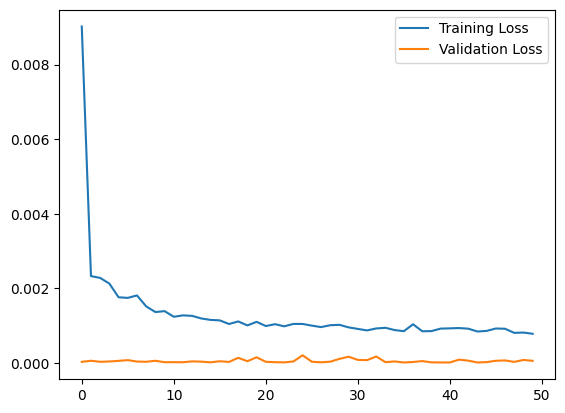
\includegraphics[width=0.8\linewidth]{Wyniki_testowe_i_walidacyjne.png}
    \caption{Wyniki testowe i walidacyjne}
    \label{fig:Wyniki_testowe_i_walidacyjne}
\end{figure}

\section{Bezpieczeństwo aplikacji}
Aplikacja wykorzystuje framework \texttt{Spring Security} w celu zapewnienia bezpieczeństwa i kontrolowania dostępu do zasobów. Dzięki zastosowaniu różnych mechanizmów uwierzytelniania i autoryzacji, takich jak \texttt{JWT} (JSON Web Tokens), oraz \texttt{Basic Authentication}, aplikacja jest chroniona przed nieautoryzowanym dostępem. Poniżej przedstawiono kluczowe komponenty zapewniające bezpieczeństwo aplikacji.\\[-10pt]

\noindent \textbf{Konfiguracja bezpieczeństwa (\texttt{SecurityConfig.java})~~}  
Pełną konfigurację bezpieczeństwa aplikacji zwiera klasa \texttt{SecurityConfig}. Definiuje ona ustawienia filtrów bezpieczeństwa, które kontrolują dostęp do zasobów. Endpointy \texttt{/client/register} i \texttt{/client/login}, służą użytkownikowi do rejestracji lub logowania, tak aby mógł mieć dostęp do platformy. 

Klasa ta zawiera również konfigurację \texttt{CORS}, która zezwala na dostęp do zasobów aplikacji z określonych domen (np. \texttt{http://localhost:3000}). Dzięki temu aplikacja ma możliwość komunikacji z frontendem.\\[-10pt]

\noindent \textbf{Generowanie i weryfikacja JWT (\texttt{JwtTokenUtils.java})~~} 
za generowanie oraz weryfikację tokenów \texttt{JWT} odpowiada klasa \texttt{JwtTokenUtils}. Tokeny te są wykorzystywane do uwierzytelniania użytkowników i zapewnienia im dostępu zasobów aplikacji. Klasa ta wykonuje następujące operacje:
\begin{itemize}
    \item Generowanie tokenów \texttt{JWT} z unikalnymi danymi użytkownika.
    \item Weryfikacja ważności tokenu, w tym sprawdzanie daty wygaśnięcia.
    \item Ustalenie, czy użytkownik w tokenie jest tym samym, który jest zapisany w bazie danych.
\end{itemize}
Po weryfikacji tokenu, użytkownik zostaje uwierzytelniony i przypisany do kontekstu bezpieczeństwa aplikacji.\\[-10pt]

\noindent \textbf{Filtrowanie tokenów JWT (\texttt{JwtAccessTokenFilter.java})~~} 
Za filtrację przychodzących żądań HTTP jest odpowiedzialna klasa \texttt{JwtAccessTokenFilter}. Filtr ten sprawdza nagłówek \texttt{Authorization} w żądaniach, aby wyodrębnić i zweryfikować token \texttt{JWT}. Jeśli token jest ważny, uzyskuje dostęp do platformy. W przypadku, gdy token jest nieważny lub nie istnieje, aplikacja zwraca odpowiedź o statusie \texttt{UNAUTHORIZED}.\\[-10pt]

\noindent \textbf{Zarządzanie danymi użytkowników (\texttt{UserInfoManager.java})~~} 
Klasa \texttt{UserInfoManager} implementuje interfejs \texttt{UserDetailsService} i jest odpowiedzialna za załadowanie użytkownika z bazy danych na podstawie nazwy użytkownika. Metoda \texttt{loadUserByUsername} korzysta z repozytorium \texttt{ClientRepository}, aby odnaleźć użytkownika, a następnie dostarcza jego dane do kontekstu bezpieczeństwa aplikacji, co pozwala na uwierzytelnianie.\\[-10pt]

\noindent \textbf{Rekordy RSA (\texttt{RSAKeyRecord.java})~~} 
Klasa \texttt{RSAKeyRecord} przechowuje klucze RSA (publiczny i prywatny), które są wykorzystywane do weryfikacji i generowania tokenów \texttt{JWT}. Klucz publiczny jest używany do weryfikacji podpisu tokenu, natomiast klucz prywatny służy do jego generowania. Jest to istotny element systemu autoryzacji, zapewniający integralność i~bezpieczeństwo transmisji danych.\\[-10pt]

\noindent \textbf{Podstawowe uwierzytelnienie (\texttt{BasicAuthenticationSecurityConfiguration.java})}
Klasa \texttt{BasicAuthenticationSecurityConfiguration} wprowadza mechanizm podstawowego uwierzytelnienia.
	
